\documentclass[../../../main.tex]{subfiles}

\begin{document}

\subsubsection{real space}

The bare Kagome lattice is a triangular Bravais lattice with a three site unit cell (called a, b and c-sites below). The Wigner Seitz-cell is a hexagon (with full symmetries, even if the drawing suggests otherwise ;) ). Geometrically speaking the lattice consists of corner-sharing equilateral triangles.


\begin{center}
	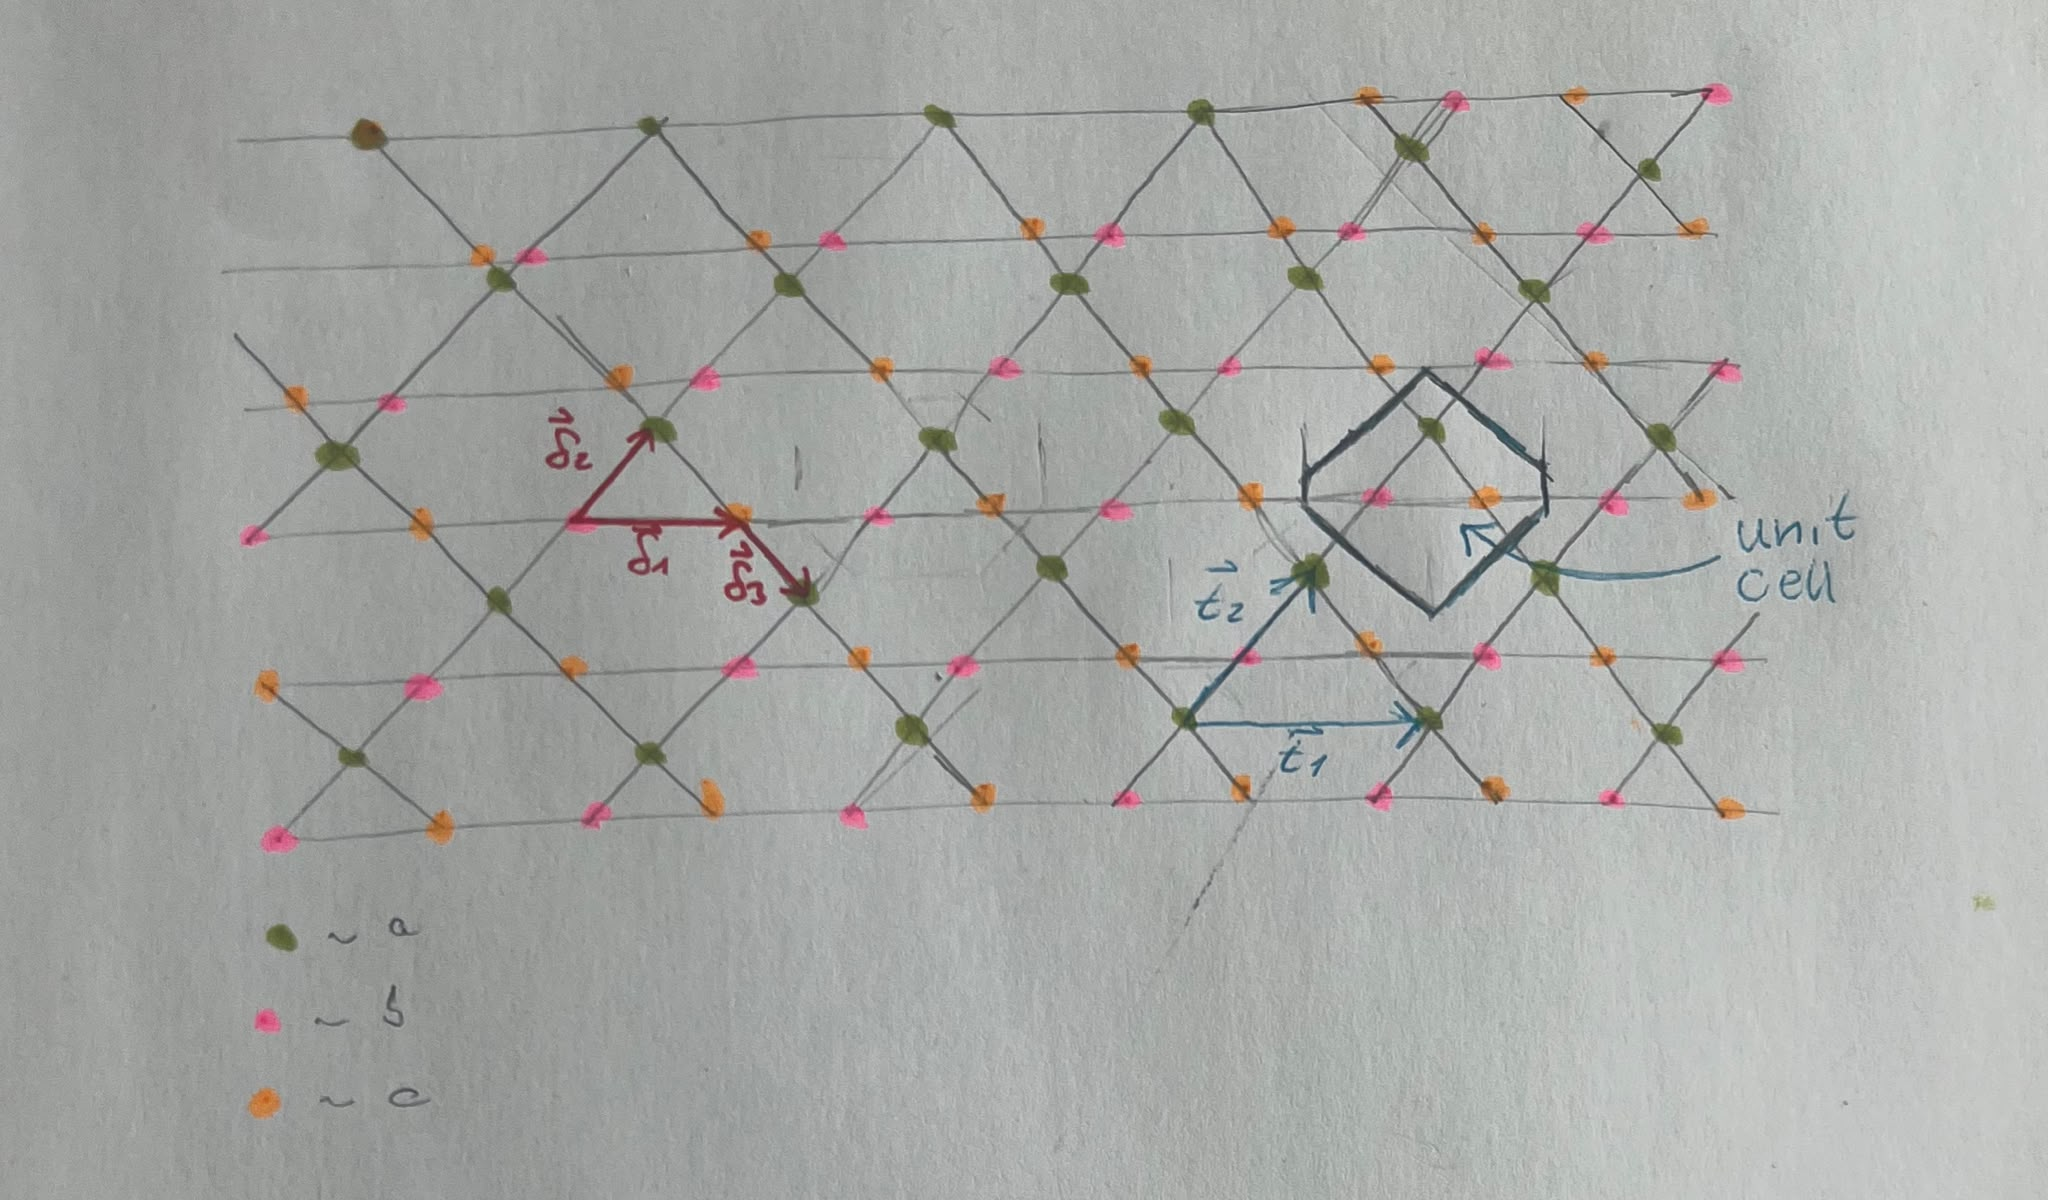
\includegraphics[width = \textwidth]{lattice-0-flux-state.jpeg}
\end{center}

In all that follows I normalize all distances wrt the distance between nearest neighbours. The nearest neighbour vectors are ( see cartoon)

\begin{equation}
	\vec{\delta}_1 = 
	\begin{pmatrix}
		1 \\
		0
	\end{pmatrix} \quad 
	\vec{\delta}_2 = \frac12
	\begin{pmatrix}
		1 \\
		\sqrt{3}
	\end{pmatrix} \quad
	\vec{\delta}_3 = \frac12 
	\begin{pmatrix}
		1 \\
		-\sqrt{3}
	\end{pmatrix}
\end{equation}

and the primitive translations 

\begin{equation}
	\vec{t}_1 = 2\vec{\delta}_1 =
	\begin{pmatrix}
		2 \\
		0
	\end{pmatrix} \quad 
	\vec{t}_2 = 2\vec{\delta}_2 =
	\begin{pmatrix}
		1 \\
		\sqrt{3}
	\end{pmatrix}.
\end{equation}

The tight binding hamiltonain is 

\begin{equation}
	H = -t \sum_{i\sigma} \left(a_{i\sigma}^\dagger c_{i\sigma} + c_{i\sigma}^\dagger b_{i\sigma} + b_{i\sigma}^\dagger a_{i\sigma} + c_{i\sigma}^\dagger b_{i+t_1;\sigma} + c_{i\sigma}^\dagger a_{i+t_1-t_2;\sigma} + a_{i\sigma}^\dagger b_{i+t_2;\sigma} + \text{h.c.}\right)
\end{equation}

The first index refers to the unit cell and the second one to the "species" of the particle, the latter being a product of the parton decomposition.

\subsubsection{reciprocal space}

The recipricoal lattice vectors are 


\begin{equation}
	\vec{b}_1 = \pi
	\begin{pmatrix}
		1 \\
		-1/\sqrt{3}
	\end{pmatrix}, \quad
	\vec{b}_2 = \pi 
	\begin{pmatrix}
		0 \\
		2/\sqrt{3}
	\end{pmatrix}
\end{equation}

The first Brillouin zone is also a hexagon (rotated by 90° wrt to the Wigner-Seitz cell). To find $H$ in reciprocal space I do a Fourier transform: 

\begin{equation}
	a_{i\sigma} = \sqrt{\frac{3}{N}} \sum_{k} e^{i\vec{k}\vec{R}_i} a_{k\sigma},
\end{equation}

where $N$ is the number of unit cells. This yields

\begin{equation}
	H = -2t \sum_{q\sigma}
	\begin{pmatrix}
		a_{q\sigma}^\dagger & b_{q\sigma}^\dagger & c_{q\sigma}^\dagger 
	\end{pmatrix}
	\begin{pmatrix}
		0 & \cos(\vec{q}\cdot\vec{\delta}_2) & \cos(\vec{q}\cdot\vec{\delta}_3) \\
		\cos(\vec{q}\cdot\vec{\delta}_2) & 0 & \cos(\vec{q}\cdot\vec{\delta}_1) \\
		\cos(\vec{q}\cdot\vec{\delta}_3) & \cos(\vec{q}\cdot\vec{\delta}_1) & 0
	\end{pmatrix}
	\begin{pmatrix}
		a_{q\sigma} \\
		b_{q\sigma} \\
		c_{q\sigma}
	\end{pmatrix}.
\end{equation}

\subsubsection{dispersion and band touching points}

The three eigenvalues are 

\begin{align}
	\varepsilon_1(\vec{q}) &= -t\left(1-\sqrt{4\cos^2(q_x)+4\cos(q_x) \cos(\sqrt{3}q_y)+1}\right) \\
	\varepsilon_2(\vec{q}) &= -t\left(1+\sqrt{4\cos^2(q_x)+4\cos(q_x) \cos(\sqrt{3}q_y)+1}\right) \\
	\varepsilon_3(\vec{q}) &= 2t,
\end{align}

see \cite{DiSante2026}. I also used 

\begin{equation}
	\cos^2\left(\frac12\left( x + \sqrt{3}q_y\right)\right) + \cos^2\left(\frac12\left(q_x - \sqrt{3}q_y\right)\right) = \cos(q_x)\cos(\sqrt{3}q_y) + 1
\end{equation}.

Interestingly, the top band is completely flat. The other two bands touch when

\begin{equation}
	\cos^2(x) + \cos(x)\cos(\sqrt{3}y) + 1/4 = 0
\end{equation}

\begin{gather}
	\Rightarrow \cos(q_x) = \frac12\left(-\cos(\sqrt{3}q_y) \pm \sqrt{\cos^2(\sqrt{3}q_y)-1}\right) \\
	\Rightarrow q_y = \frac{\pi l}{\sqrt{3}}, \; l \in \mathbb{N} \\
	\Rightarrow q_x = (-1)^s\left(\frac{\pi}{2} + \frac{(-1)^{l}\pi}{6}\right) + 2\pi m , \; m \in \mathbb{N}, \; s \in [0,1]
\end{gather}

These touching points lie at the corners of the Brillouin zone, there are two "species". \textcolor{red}{One can imagine that two of the parameters represent translation by recprocal lattice vectors whil the third one selects the species of the touching points. This not what m, l and s do but maybe one can transform them. Also, why does the solution depend on three parameters?}  For example 

\begin{align}
	\vec{K} &= 
	\begin{pmatrix}
		2\pi/3 \\
		0
	\end{pmatrix}, \quad m=0, s=0, l = 0 \\
	\vec{K}^\prime &= 
	\begin{pmatrix}
		-2\pi/3 \\
		0
	\end{pmatrix}, \quad m = 0, s = 1,  l = 0.
\end{align}

\subsubsection{filling factor}

\textcolor{red}{The idea is the follwing: The lower two bands contain the same number of states by symmetry. By calculating the number of states of the upper band (should be easy) it shoulb possible to calcualte at what filling factor the low energy physics happen exactly the linear touching points.}

\subsubsection{linearization in reciprocal space}

Use

\begin{equation}
	\cos(\left(\vec{K}^{(\prime)}+\vec{p}\right)\cdot\vec{\delta}_{ij}) \approx \cos(\vec{K}^{(\prime)}\cdot\vec{\delta}_{ij}) - \sin(\vec{K}\cdot\vec{\delta}_{ij})\left(\vec{p}\cdot\vec{\delta}_{ij}\right)
\end{equation}


and

\begin{align}
	\begin{split}
		\vec{K}\cdot\vec{\delta}_{1} &= \frac{2\pi}{3} \\
		\vec{K}\cdot\vec{\delta}_{2} &= \frac{\pi}{3} \\
		\vec{K}\cdot\vec{\delta}_{3} &= \frac{\pi}{3} \\
		\vec{K}^\prime &= - \vec{K}
	\end{split}
\end{align}


\begin{align}
	H(\vec{K}) \approx -t\sum_{p\sigma}
	\begin{pmatrix}
		a_{p\sigma}^\dagger b_{p\sigma}^\dagger c_{p\sigma}^\dagger
	\end{pmatrix}
	\begin{pmatrix}
		0 & 1-\sqrt{3}\vec{p}\cdot\vec{\delta}_2 & 1 - \sqrt{3}\vec{p}\cdot\vec{\delta}_3 \\
		1-\sqrt{3}\vec{p}\cdot\vec{\delta}_2 & 0 & -1-\sqrt{3}\vec{p}\cdot\vec{\delta}_1 \\
		1-\sqrt{3}\vec{p}\cdot\vec{\delta}_3 & -1-\sqrt{3}\vec{p}\cdot\vec{\delta}_1 & 0
	\end{pmatrix}
	\begin{pmatrix}
		a_{q\sigma} \\
		b_{q\sigma} \\
		c_{q\sigma}
	\end{pmatrix}
\end{align}

\end{document}
